% -----------------------------------------------------------------------------
%   Arquivo: ./02-elementos-textuais/trabalhosRelacionados.tex
% -----------------------------------------------------------------------------

\chapter{Aprendizado de Máquina}
\label{chap:MachineLearning}

\section{Formulação e Caracterização do Aprendizado de Máquina}

Nos primórdios da inteligência artificial, pesquisadores foram capazes de resolver problemas que são intelectualmente difíceis para os seres humanos, mas relativamente simples para os computadores. Exemplo disso são os problemas que podem ser descritos por uma sequência de regras ou que podem ser solucionados por operações matemáticas \cite{Goodfellow-et-al-2016}.

A dificuldade surgiu para fazer com que os computadores fossem capazes de resolver tarefas fáceis para os humanos, mas difíceis de serem descritas de forma algorítmica, como reconhecer escrita, identificar rostos em imagens ou ainda definir regras de decisão de forma autônoma \cite{Goodfellow-et-al-2016}.

Eis que surgiu o campo de Aprendizado Máquina, uma alternativa que permitia computadores aprender por exemplo e não por regras. Ao reunir o conhecimento da experiência, esta abordagem evita a necessidade de operadores humanos especificar formalmente todo o conhecimento que o computador precisa. Isso ocorre através da combinação do aprendizado de conceitos simples, em formato pré-definido, combinados de forma hierárquica para formar um aprendizado de conceitos complicados \cite{Goodfellow-et-al-2016}.

Segundo \citeonline{Cherkassky2007}, o processo de aprendizado é definido como a estimação de uma relação ou estrutura, previamente desconhecida, entre entrada e saída. Segundo o autor, o processo de aprendizado normalmente envolve três componentes \ref{fig:MLFormulation} : o \textit{Gerador} de amostras, um \textit{Sistema} que gera as saídas reais e o \textit{Aprendizado de Máquina} que estima a relação desconhecida entre entrada e saída. 

\begin{figure}[!htb]
	\centering
	\caption{Formulação do Aprendizado} 
	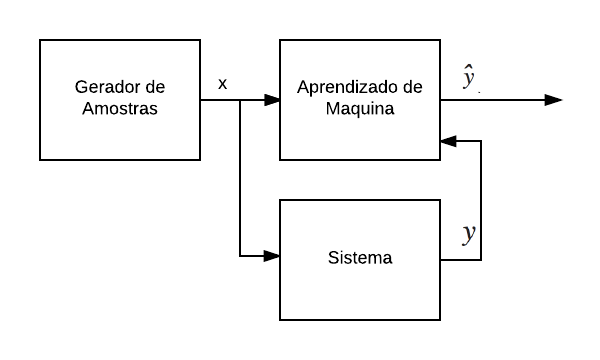
\includegraphics[width=0.8\textwidth]{./04-figuras/MLForm.png}
	\label{fig:MLFormulation}
\end{figure}

\citeonline{Cherkassky2007} explica que o \textit{Gerador} produz aleatoriamente, com distribuição de probabilidade $p(x)$, vetores $x \in {\mathbb {R}} ^{n}$, que são as características. O \textit{Sistema} é capaz de produzir, com probabilidade $p(y | x)$, saídas $y = g(x) + \epsilon$ em que $\epsilon$ é um ruido branco de $\mu = 0$. De forma geral, o \textit{Aprendizado de Máquina} é capaz de implementar uma função $\hat{y} = f(x, \omega)$, $\omega \in \Omega$, em que $\Omega$ é conjunto de parâmetros da função $f$.

O aprendizado de máquinas clássico diz respeito à aprender pelo exemplo, que é definido como um conjunto de dados, previamente obtidos pelo \textit{Gerador} e \textit{Sistema}, composto por variáveis quantitativas e qualitativas que são características do problema. Na situação onde existe uma variável resposta, o aprendizado é chamado de supervisionado, na situação onde essa variável não existe, o problema é definido como aprendizado não supervisionado. A figura \ref{fig:MLProblems} ilustra essa taxonomia, bem como algumas de suas sub-divisões.


\begin{figure}[!htb]
	\centering
	\caption{Principais Problemas em Aprendizado de Máquina} 
	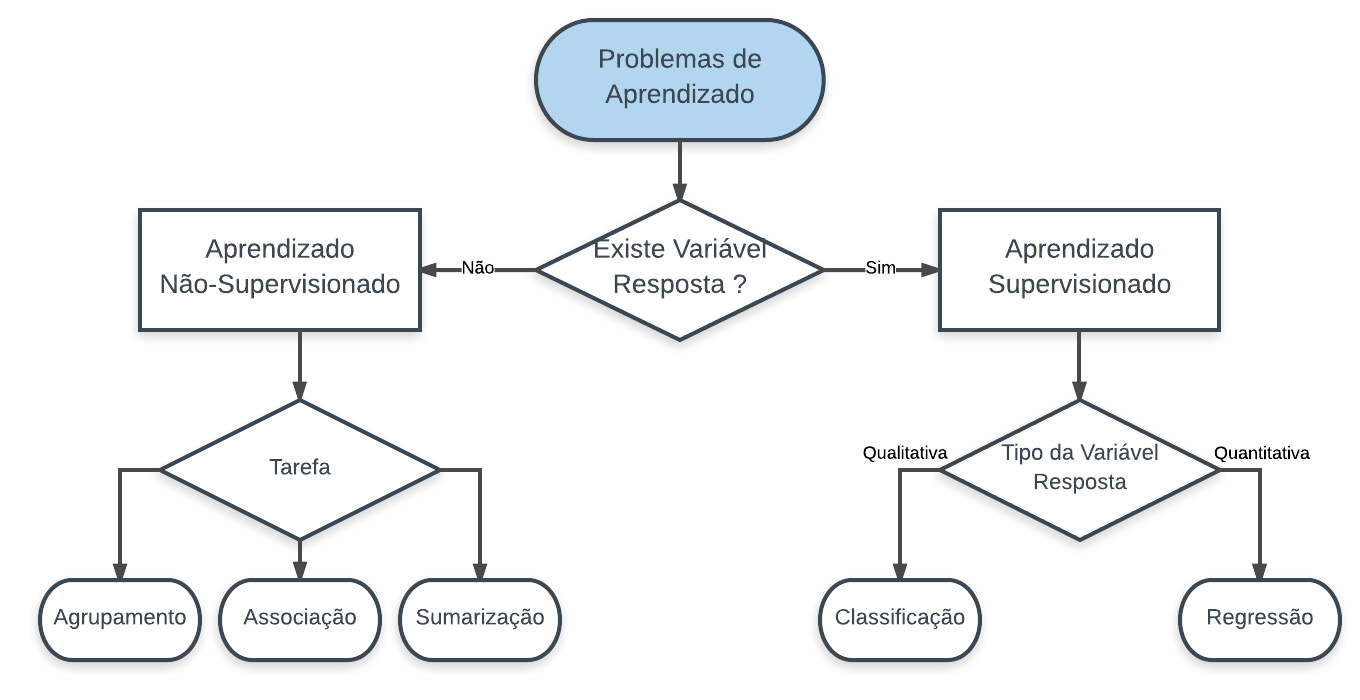
\includegraphics[width=0.8\textwidth]{./04-figuras/MLProblems.png}
	\label{fig:MLProblems}
\end{figure}
\section{Aprendizado Supervisionado}

No aprendizado supervisionado, o objetivo é prever o valor de uma variável resultado com base em variáveis características. Na situação que a variável resposta é quantitativa, o problema é considerado como uma tarefa de regressão. Quando essa variável resposta é quantitativa, a tarefa é chamada de classificação.

De acordo com \citeonline{Cherkassky2007}, existem duas interpretações para o problema de aprendizado : identificação e imitação. A interpretação escolhida para fundamentar esse trabalho é a de imitação, descrita por \citeonline{Vapnik1971}.

O objetivo do aprendizado é encontrar uma função $f(x, \omega)$ que aproxima, da melhor forma possível, a saída $y$ do \textit{Sistema}. Para formular esse problema matematicamente, \citeonline{Cherkassky2007}, assumem pares de características e respostas, $(x_i, y_i)$ em que $i = (1, 2, ..., n)$ e $ n \in \mathbb {N}$, e uma função de custo $L(y, f(x, \omega))$que mede a discrepância entra saída do \textit{Sistema} $y$ e do \textit{Aprendizado de Máquina} $\hat{y}$. Então, formulam que a tarefa do aprendizado é descrita pela equação \ref{eq:LearningEq} . 

\begin{equation}
{	
	{\displaystyle {\underset {f}{\operatorname {arg\,min} }}\, L(y, f(x, \omega))}
}
\label{eq:LearningEq}
\end{equation}

A principal diferença entre problemas de classificação e regressão é a função de custo. Como a variável de saída de cada um desses problemas tem um formato diferente, a função de custo deve ser adaptada especificadamente para ele. Contudo, a formulação do aprendizado feito na equação \ref{eq:LearningEq} permanece inalterada, pois o objetivo é sempre minimizar a discrepância entre \textit{Sistema} e \textit{Aprendizado de Máquina} \cite{Cherkassky2007}.

\subsection{Problemas de Classificação}
A situação mais simples de classificação é aquele em que a saída $y$ assume apenas dois valores, $y = 0$ ou $y = 1$, em que é chamada de problema de classificação binária. Nessa situação, a função de custo específica é do formato \ref{eq:ClassProb}.

\begin{equation}
{	
	 L(y, f(x, \omega)) = \begin{dcases*}
	0,  & se $y = f(x, \omega)$ \\
	l,  & se $y \ne f(x, \omega)$ 
	\end{dcases*} \\ 
	l \in \mathbb {R^+}
}
\label{eq:ClassProb}
\end{equation}

O senário em que $y$ assume $q$ valores, em que $q > 2 \land q \in \mathbb {N}$, pode ser simplificado em $q$ problemas de classificação binária em que o problema $j$ tem forma $y = j \rightarrow y_j = 1$ e $y_j \neq  \rightarrow y_j = 0 $, para $ 0 \leq j \leq q \land j \in \mathbb {N}$.

\subsection{Problemas de Regressão}
O problema de regressão é caracterizado por $y \in \mathbb {R}$, dessa forma a função de custo normalmente é formulada como mostra a equação \ref{eq:RegProb}, onde $d$ é uma métrica genérica de distância entre dois números reais.

\begin{equation}
L(y, f(x, \omega)) = d(y, f(x, \omega))
\label{eq:RegProb}
\end{equation}

\section{Aprendizado Não Supervisionado}

O aprendizado não supervisionado é caracterizado pela não existência de uma variável resposta $y$. Contudo, os problemas dessa tarefa podem ser divididos em três grandes grupos : agrupamento, associação e sumarização. Será discutido nessa seção apenas a tarefa de agrupamento, porque é a única que será contemplada pelo projeto final de software.

\subsection{Agrupamento}
A tarefa de agrupamento, diz respeito a atribuição de rótulos para amostras de forma que aquelas com rótulos iguais possuam mais similaridades entre sí do que entre aquelas com rótulos diferentes. 

Não existe uma padronização, entre autores, na classificação das metodologias para realizar essa tarefa. Porém, segundo \citeonline{berkhin2006survey}, eles podem ser divididos em três grandes grupos :
\begin{compactitem}
	\item \textbf{Hierárquicos :} São modelos baseados em agrupar amostras hierarquicamente, por meio de uma função de similaridade. 
	
	\item \textbf{Baseado em densidade :} São modelos que utilizam a ideia de que agrupamentos estão definidos por amostras em regiões densas do espaço.
	
	\item \textbf{Baseado em partição :} São modelos que particionam o espaço amostral em regiões, normalmente esses métodos são formulados por otimização iterativa e incluem os algorítimos baseados em centros e distribuições de probabilidade.
	
\end{compactitem}
%
%\subsection{Associação}
% As regras de associação é um campo que surgiu para resolver o problema do \textit{'carrinho de compras'} de bases de dados comerciais, com o objetivo de encontrar relações interessantes entre variáveis diferente um conjunto de dados muito grande \cite{Hastie2009, Agrawal1993}.  
%
%\subsection{Sumarização}
%
